
\documentclass[Recitation10_Review.tex]{subfiles}

\section{Externalities}

\begin{frame}{Externalities: Basic Concepts}
	\begin{itemize}
		\item Individual actions create an effect to agents that \textit{external} to the decision;
		\item \textit{Positive} if the effect increases others' utility, \textit{negative} otherwise;
		\item Policy criterion: we use additive welfare, sum of all agents' utilities;
		\item Policy issue: if agents decide \textit{in isolation}, the supply of the good in question is sub-optimal:
		\begin{itemize}
			\item Negative externality: excess supply. Example: pollution; an individual firm might pollute so much that the individual gains in terms of profits are outweighed by \textit{collective losses};
			\item Positive externality: insufficient supply. Example: R\&D; an individual firms' research can benefit other firms. \textit{Collective benefits} are larger than private in isolation. 
		\end{itemize}
	\item Remedies:
	\begin{itemize}
		\item Coase theorem: define property rights, but need \textit{costless bargaining};
		\item Impose quotas: always feasible, but need a lot of info;
		\item Pigouvian taxation: tax negative ext. goods, subsidize positive ext. goods.
	\end{itemize}
	\end{itemize}
\end{frame}

\begin{frame}{Pollution example (negative externality)}
	A firm produces x polluting goods, maximizing profits:
	\[
		\Pi(x) = x - b\cdot x^2 \Rightarrow x^\ast = \dfrac{1}{2b}
	\]
	However, for the community there is the following loss from pollution:
	\[
		C(x) = -c \cdot x^2.
	\]
	Social (utilitarian/additive) welfare, maximized by social planner:
	\[
		W(x) = \Pi(x) + C(x) = x - b\cdot x^2 -c \cdot x^2. \Rightarrow x^{\text{pl}} = \dfrac{1}{2(b+c)}.
	\]
	There is over-supply of polluting goods since $x^{\text{pl}} < x^\ast$. 
\end{frame}




\begin{frame}{Solving Externalities}
The aim is to make the firm \textit{internalize} the negative effects. Three ways to go about it:
\begin{enumerate}
	\item Coase theorem: give property rights to the community, firm has to pay $p^x$ to the community in order to produce each unit of $x$. If actually no bargaining (one consumer) community sets:
	\[
		U(x) = C(x) + p^xx= 0 \rightarrow p^x = cx.
	\]
	\item Impose a cap: the planner directly sets cap $\bar{x} = x^{\text{pl}}$;
	\item Pigouvian tax: impose a tax $\tau^x$ per unit of $x$ such that $\Pi(x) - \tau^x\cdot x= W(x)$. Solution: $\tau^x= cx$ (like in Coase case).
\end{enumerate}
General Steps:
\begin{itemize}
	\item Set up individual problem (like $\Pi(x)$ in example) and optimal quantities $x^\ast$;
	\item Set up the planner problem. Write down \textit{social} welfare, $W(x)$ as sum of individual utilities of \textit{entire society}, solve for quantity that maximizes \textit{social welfare}. This is the planner's solution $x^{\text{pl}}$;
	\item Find \textit{policy instrument} to make  $x^\ast=x^{\text{pl}}$. With this instrument, the individual function of whoever is choosing $x$ must coincide with social welfare $W(x)$.
\end{itemize}

\end{frame}


\section{Insurance}


\begin{frame}{Expected Utility: Basic Concepts}
\begin{itemize}
	\item Agents now evaluate different risky scenarios, choosing \textit{lotteries} instead of goods;
	\item Recall: lotteries $L$ are a set of \textit{probabilities} with associated payoffs, e.g.:
	\[
		L=\begin{cases}
		x_1 \ \text{w.p.} \ p_1\\
		x_2 \ \text{w.p.} \ p_2
		\end{cases}.
	\]
	\item VnM theorem tells us that---subject to assumptions---agents evaluate lotteries using the \textit{expected utility of outcome $x$}:
	\[
		U(L) = \sum_{j=1}^{n} p_j u(x_j) \equiv E[u(x)].
	\]
\end{itemize}
\end{frame}

\begin{frame}{Insurance}
	Define the \textit{expected outcome} as the expectation of $x$ (average $x$ that agent gets):
	\[
		E(x) = \sum_{j=1}^{n} p_j x_j.
	\]
	This yields utility $u(E(x))$. We can then define the \textit{certainty equivalent} corresponding to the lottery, as $CE(L)$ such that:
	\[
		u(CE(L)) = E\left[u(x)\right].
	\]
	This gives how much the agent is \textit{willing to pay} in order to avoid risk and be indifferent to the situation with risk. Three cases with associated convexities (comes from Jensen's inequality):
	\begin{itemize}
		\item $CE(L)>E[x]$: risk-averse IFF  $E\left[u(x)\right] < u(E[x])$ IFF $u(x)$ is concave;
		\item $CE(L)=E[x]$: risk-neutral IFF  $E\left[u(x)\right] =u(E[x])$ IFF $u(x)$ is linear;
		\item $CE(L)>E[x]$: risk-loving IFF  $E\left[u(x)\right] >u(E[x])$ IFF $u(x)$ is convex.
	\end{itemize}
Risk-averse individuals will want to \textit{pay} (reduce their expected wealth) to avoid risk, generating \textit{demand for insurance}.
\end{frame}

\begin{frame}{How much insurance?}
General form: agents pay a premium $p$ per unit of money received in a certain state and a fixed fee $F$ to buy into insurance. Both are paid \textit{regardless of the state that occurs}. Suppose there are two states, good, and bad (where insurance pays). Utility without insurance (w.p of good event $\pi^G$):
\[
	E(u(x)) = \pi^Gu(x^G) + (1-\pi^G)u(x^B).
\]
Utility with insurance $I$:
\[
	E(u(x)) =\max_{I\geq0} \pi^Gu\left[x^G - p\cdot I - F\cdot\mathbf{1}\left(I>0\right)\right] + (1-\pi^G)u\left[x^B - p\cdot I + I - F\cdot\mathbf{1}\left(I>0\right)\right].
\]
Split into two parts:
\begin{enumerate}
	\item Assuming I take positive insurance and pay $F$, what $I$ would I set? Maximize expected utility in $I$ and find solution $I^\ast$.
	\item If I found the $I^\ast>0$, is the expected utility with insurance and fee $F$ at least as large as the utility without? If yes, I will purchase insurance $I^\ast>0$, otherwise no insurance.
\end{enumerate}

\end{frame}

\begin{frame}{Example}
	\[
		x=\begin{cases}
		1\ \text{w.p.} \ \pi\\
		2 \ \text{w.p.} \  (1-\pi)
		\end{cases}.
	\]
	Insurance available at cost $p$ per unit insured and fee $F$, utility is $u(x) = \sqrt{(x)}$. Suppose I buy $I^\ast>0$
	\[
		E\left[u(x)\right] = \max_{I>0} \pi \sqrt{(1 +(1-p) I - F)} + (1-\pi) \sqrt{(2 -pI - F)}.
	\]
	Suppose insurance is \textit{actuarially fair}, that is insurance company does not make profits in expectation:
	\[
		\pi(1-p) = (1-\pi)p \ \Rightarrow \dfrac{p}{1-p} = \dfrac{\pi}{1-\pi} \Rightarrow c =  p.
	\]
	Then, FOC:
	\[
		\pi(1-\pi)\sqrt{(1 +(1-\pi) I - F)} = \pi(1-\pi)\sqrt{(2 -\pi I - F)} \Rightarrow 1 +(1-\pi) I - F= 2 -\pi I - F
	\]
	Which implies $I^\ast = 1$, \textbf{full insurance}.
\end{frame}

\begin{frame}{Example cont.}
We found:
\[
	I^\ast =  1.
\]
Regardless of $F$. Now we have to figure out whether the agent will purchase it. Note that, with full insurance, the agent now gets a fixed wealth $2 - p - F$ regardless of the state!\\

Purchase will then occur if and only if:
\[
	2 - \pi - F \geq CE \ \text{s.t.} \ u(CE) = E\left[u(x)\right].
\]
Find CE:
\[
	\sqrt{CE} = \pi\sqrt{1} + (1-\pi) \sqrt{2} \Rightarrow CE = \left(\pi +(1-\pi) \sqrt{2}  \right)^2 
\]
So we obtain:
\[
	F\leq 2 - \pi -CE = 2 - \pi - \left(\pi +(1-\pi) \sqrt{2}  \right)^2
\]
In words: the agent is willing to pay all the expected wealth in excess of the certainty equivalent!

\end{frame}


\begin{frame}{Insurance Recap}
	\begin{itemize}
		\item If insurance is \textit{actuarially fair} (no profits from \textit{premium part} of the insurance), a risk averse agent will buy \textbf{full insurance}, conditional on fee not being too high.
		\item If full insurance is purchased, wealth is fixed at some level $I^\text{ins}$.
		\item Insurance can charge a fee $F = x^\text{ins} - CE$, where $x^\text{ins}$ is the certain wealth that the agent has with insurance.
		\item Intuition: by definition, the agent is indifference between the lottery \textit{without insurance} and receiving CE w.p. 1.
		\item Thus, the insurance can capture all the surplus that the agent is getting from the insurance contract, by giving the agent their certainty equivalent on average.
	\end{itemize}
\end{frame}

\section{Signaling games}

\begin{frame}{Games: Nash Equilibrium}
	Basic concept of equilibrium: we are in an equilibrium if no agent would be better off changing their action, given what the other agent does. Simple example:
	\begin{center}
		\begin{tabular}{l| c| c}
			Agent 1/Agent 2 & Action 1 & Action 2\\
			Action 1 & 0,0 & 1,-1 \\
			Action 2 & -1,1 & -1, -1 
		\end{tabular}
	\end{center}
	Choose an action without knowing what the other agent does, so I have to define a policy \textit{conditional on each of the actions}. Suppose I am agent 1.
	\begin{itemize}
		\item If Agent 2 chooses Action 1, I would want to choose Action 1;
		\item If Agent 2 chooses Action 2, I would want to choose Action 1 again. 
	\end{itemize}
	In light of my choices, what will agent 2 do? She knows that:
	\begin{itemize}
		\item If she chooses Action 1, she gets $0$;
		\item If she chooses Action 2, she gets $-1$.
	\end{itemize}
	Thus, what is an equilibrium? It is the pair (Action 1, Action 1). Why? Nobody wants to deviate from their policies.
\end{frame}


\begin{frame}{Signaling Games}
\begin{itemize}
	\item Same concept of equilibrium: everybody is choosing their \textit{optimal response} to what everybody else is doing (no-deviation principle);
	\item But actions are now \textit{a signal acquisition} for the \textit{sender} and a \textit{screening rule} for the receiver;
	\item Education example: \textit{senders} are the types, who can acquire the costly education signal; \textit{receivers} are the employers who have to choose a \textit{wage rule} to maximize their profits given the signal they observe.
	\item Equilibrium in education:
	\begin{enumerate}
		\item  amount of education is consistent \textit{with the screening policy of the employer}: no agent wants a different amount of education than what they are acquiring;
		\item  policy of the employer is consistent  with \textit{the signals acquired by the market}: if employer is giving a different wage according to the signal, she does not want to switch to a flat wage, and vice versa.
	\end{enumerate}
\end{itemize}

\end{frame}


\begin{frame}{Equilibrium in Signaling Games}
\begin{itemize}
	\item Two \textit{types} of equilibria:
	\begin{enumerate}
		\item Pooling: everyone does the same thing;
		\item Separating: agents choose signals that \textit{separate} them into groups, so at least one agent does something differently from the others.
	\end{enumerate}
\item Pooling in education: employer must not attach value to the education that workers would find convenient to attain (we will discuss this below). Simplest case:
\begin{enumerate}
	\item Employer offers wage = average productivity in population. Outside option is getting 0 profits;
	\item  Nobody acquires education because it is costly and not valued;
	\item Given that nobody acquires 0 education, the employer will hire random workers and on average make
	\[
		\text{profits} = \text{average productivity} - \text{wage} = 0.
	\]
	\item This makes sense, the employer makes profits equal to the outside option. Since nobody acquires education, she does not want to offer a wage that depends on education.
\end{enumerate}
\end{itemize}
\end{frame}

\begin{frame}{Separating: all you need is this graph}
Recall: $\lambda$ is the share of agents with productivity $Y=2$, others have $Y=1$. 
	\begin{figure}
		\centering
		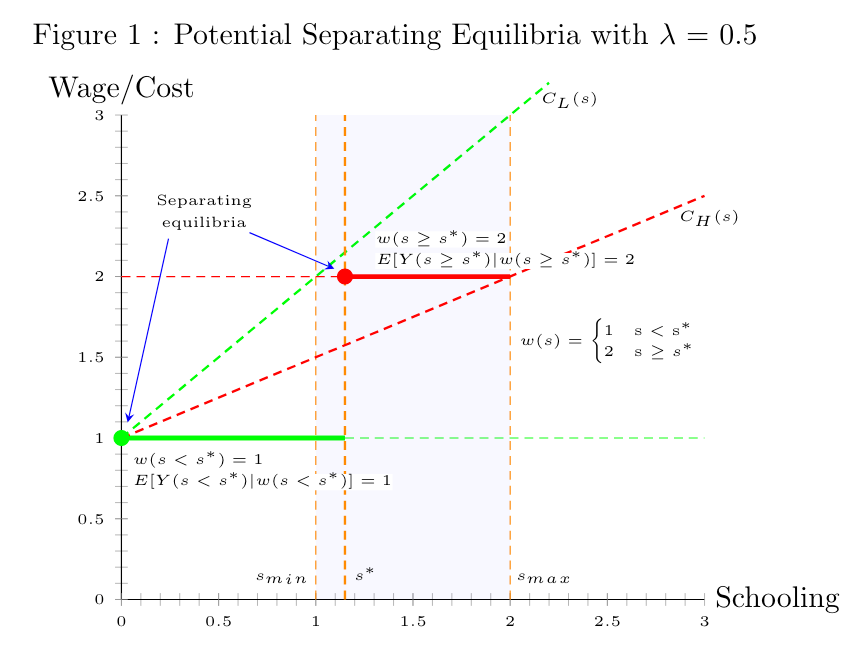
\includegraphics[width=0.65\linewidth]{Figures/SepGraph}
		\caption{}
		\label{fig:sepgraph}
	\end{figure}
\end{frame}


\section{Market for lemons}

\begin{frame}{Market for lemons}
Idea is the same as before, however now the signal is the \textbf{price} and it is \textit{costless to acquire}, so the only equilibrium is a \textbf{pooling equilibrium}:
\begin{itemize}
	\item Buyer offer the same price to all sellers;
	\item Sellers charge the same price.
\end{itemize}
Equilibrium has to satisfy two conditions:
\begin{enumerate}
	\item Demand equals supply at equilibrium price;
	\item Price is such that consumer gets the average value of good supplied and sellers actually want to supply goods with that average quality.
\end{enumerate}
Separating alternative: Full disclosure, i.e. everyone reveals their quality. Only if:
\begin{itemize}
	\item the signal is credible;
	\item the signal is costless.
\end{itemize}
If either fails, you will have at least some extent of pooling.
\end{frame}


\begin{frame}{Market Unraveling}
	With this term, we indicate a case where:
	\begin{itemize}
		\item \textit{a pooling equilibrium cannot be supported by any price};
		\item therefore, only bad-quality good will be sold in equilibrium. 
	\end{itemize} 
Example: quality can be 1 or 0, with equal probability. Price if both are supplied: .5.\\
A zero-quality good has supply
\[
	Q_0(p) = p - .2 \rightarrow Q(.5) = .3,
\]
while a one-quality good has supply
\[
	Q_1(p) = p - .5. \rightarrow Q_1(.5) = 0.
\]
But then the only price that makes sense is $0$ (only zero-quality goods are supplied). The market unravels completely (in this case to the point of not existing, nobody sells or buys anything).
\end{frame}

\begin{frame}{Econometric Methods}
	\begin{itemize}
		\item Instrumental variables (Feyrer, 2009; Autor et al., 2013). 
		\begin{itemize}
			\item Idea: solve endogeneity issues by using a variable $Z$ that does not affect the outcome $Y$ directly, but only shifts the endogenous variable interest $X$;
			\item Assumption: $Z$ only affects $Y$ \textit{through its effect on} $X$, and \textit{no other channels}.
		\end{itemize}
		\item Regression discontinuity (Tyler et al., 2000), assumption is very similar to an instrumental variable: 
		\begin{itemize}
			\item Idea: solve endogeneity issues by using a \textit{running} variable $Z$ that, around a specific cutoff $\bar{Z}$ (GED score), does not affect the outcome $Y$ directly, but only shifts the endogenous variable interest $X$ (GED acquired);
			\item Assumption 1: if $\bar{Z}$ was not chosen to be a cutoff, units with $Z$ in a close neighborhood of the cutoff would be indistinguishable in their outcomes $Y$ and other covariates (no other effect of $Z>\bar{Z}$ on $Y$ other than change in $X$);
			\item Assumption 2: units cannot self-select on either side of the cutoff (also no other effect of $Z>\bar{Z}$ on $Y$ other than change in $X$; if people could choose, the outcomes $Y$ would likely change discretely around the cutoff).
		\end{itemize}
	\end{itemize}
Cool visualizations (website is old but gold): \url{http://www.nickchk.com/causalgraphs.html}
\end{frame}